% !TeX TXS-program:compile = txs:///arara
% arara: pdflatex: {shell: no, synctex: no, interaction: batchmode}
% arara: pdflatex: {shell: no, synctex: no, interaction: batchmode}

\documentclass[11pt,a4paper]{ltxdoc}
\usepackage{bera}
\usepackage{inconsolata}
\usepackage[T1]{fontenc}
\usepackage[utf8]{inputenc}
\usepackage[scale=0.875]{cabin}
\usepackage{calculatoritems}
\usepackage{fancyvrb}
\usepackage{fancyhdr}
\usepackage{tabularray}
\usepackage{fontawesome5}
\fancyhf{}
\renewcommand{\headrulewidth}{0pt}
\lfoot{\sffamily\small [calculatoritems]}
\cfoot{\sffamily\small - \thepage{} -}
\rfoot{\hyperlink{matoc}{\small\faArrowAltCircleUp[regular]}}
\usepackage{hologo}
\providecommand\tikzlogo{Ti\textit{k}Z}
\providecommand\TeXLive{\TeX{}Live\xspace}
\let\TikZ\tikzlogo

\usepackage{hyperref}
\urlstyle{same}
\hypersetup{pdfborder=0 0 0}
\usepackage[margin=2cm]{geometry}
\setlength{\parindent}{0pt}
\def\TPversion{0.1.3}
\def\TPdate{03/02/2025}
\usepackage{enumitem}
\usepackage{tcolorbox}
\usepackage{pgffor}
\tcbuselibrary{breakable,skins,hooks,listingsutf8}

\lstdefinestyle{packagestyle}
{
	language=[LaTeX]TeX,%
	columns=fullflexible,%
	extendedchars=true,%
	basicstyle=\small\ttfamily,%
	keywordstyle={\color{black}},%
	classoffset=0,%
	keywords={\includegraphics},%
	alsoletter={-},%
	keywordstyle={\color{blue}},%
	classoffset=1,%
	alsoletter={-},%
	morekeywords={},%
	keywordstyle={\color{violet}},%
	classoffset=2,%
	alsoletter={-},%
	morekeywords={calculatoritems,\CalcItemMenu,\nwkstri,\tidots,\casiodots,\CalcKey,\CalcKeyNwks,\fontkeyNWKS,\fontkeyCASIOcw,\fontkeyCASIOfx,\CalcKeyCasioCW,\CalcKeyCasioFX,\CalcKeyTI,\CalcKeyTIfr,\fontkeyTIfr,\fontkeyTI,\inckeycalc},%
	keywordstyle={\color{green!50!black}},%
	classoffset=3,%
	morekeywords={xelua,noamssymb,model,type,fsep,font,len,bg,rightsymb,colorfont},%
	keywordstyle={\color{orange}},%
	inputencoding=utf8/latin1
}

\lstset{
%	language=[LaTeX]TeX,%
	basicstyle=\small\ttfamily,%
	keywordstyle={},%
%	classoffset=0,%
%	keywords={},%
%	alsoletter={-},%
%	keywordstyle={\color{blue}},%
%	classoffset=1,%
%	alsoletter={-},%
%	morekeywords={},%
%	keywordstyle={\color{violet}},%
%	classoffset=2,%
%	alsoletter={-},%
%	morekeywords={calculatoritems,\CalcItemMenu,nwkstri,tidots,casiodots},%
%	keywordstyle={\color{green!50!black}},%
%	classoffset=3,%
%	morekeywords={xelua,noamssymb,model,type,fsep,font,len,bg,rightsymb},%
%	keywordstyle={\color{orange}}
}

\newtcblisting{DemoCode}[1]{%
	enhanced,width=\linewidth,%
	bicolor,size=title,%
	colback=cyan!10!white,%
	colbacklower=cyan!5!white,%
	colframe=cyan!75!black,%
	listing options={%
		breaklines=true,%
		breakatwhitespace=true,%
		style=packagestyle,%
		basicstyle=\footnotesize\ttfamily,%
		tabsize=4,%
		commentstyle={\itshape\color{gray}},
		keywordstyle={\color{blue}},%
		classoffset=0,%
		keywords={\newfontfamily,\includegraphics},%
		alsoletter={-},%
		keywordstyle={\color{blue}},%
		classoffset=1,%
		alsoletter={-},%
		morekeywords={\CalcItemMenu,\nwkstri,\tidots,\casiodots,\CalcKey,\CalcKeyNwks,\fontkeyNWKS,\fontkeyCASIOcw,\fontkeyCASIOfx,\CalcKeyCasioCW,\CalcKeyCasioFX,\CalcKeyTI,\CalcKeyTIfr,\fontkeyTIfr,\fontkeyTI,\inckeycalc},%
		keywordstyle={\color{violet}},%
		classoffset=2,%
		alsoletter={-},%
		morekeywords={calculatoritems,\CalcItemMenu,\nwkstri,\tidots,\casiodots,\CalcKey,\CalcKeyNwks},%
		keywordstyle={\color{green!50!black}},%
		classoffset=3,%
		morekeywords={xelua,noamssymb,model,type,fsep,font,len,bg,rightsymb,colorfont},%
		keywordstyle={\color{orange}}
	},%
	#1
}

\newtcbinputlisting\DemoCodeFile[1]{%
	enhanced,width=\linewidth,%
	bicolor,size=title,%
	colback=lightgray!10!white,%
	colbacklower=lightgray!5!white,%
	colframe=lightgray!75!black,%
	listing options={%
		breaklines=true,%
		breakatwhitespace=true,%
		style=tcblatex,
		extendedchars=true,%
		basicstyle=\tiny\ttfamily,%
		keywordstyle={},%
		tabsize=2,%
		commentstyle={\itshape\color{gray}},%
		inputencoding=utf8/latin1
	},%
	breakable,
	listing only,%
	listing file={#1}
}

\NewDocumentCommand\ShowCode{ m }{%
	\colorbox{lightgray!50}{\lstinline!#1!}%
}

\begin{document}

\thispagestyle{empty}

\begin{center}
	\begin{minipage}{0.88\linewidth}
		\begin{tcolorbox}[colframe=yellow,colback=yellow!15]
			\begin{center}
				\renewcommand{\arraystretch}{1.25}%
				\begin{tabular}{c}
					{\Huge \texttt{calculatoritems}}\\
					\\
					{\LARGE Insert items (or simple keys)} \\
					{\LARGE of classic calculators.} \\
					\\
					{\small \texttt{Version \TPversion{} -- \TPdate}}
				\end{tabular}
			\end{center}
		\end{tcolorbox}
	\end{minipage}
\end{center}

\begin{center}
	\begin{tabular}{c}
		\texttt{Cédric Pierquet}\\
		{\ttfamily cpierquet -- at -- outlook . fr}\\
		\texttt{\url{https://forge.apps.education.fr/pierquetcedric/packages-latex}} \\
	\end{tabular}
\end{center}

\hrule

\vfill

\begin{tcblisting}{colframe=lightgray,colback=lightgray!5,listing only}
Classic calculators items or menus:

35+E:
  \CalcItemMenu[model=35+,font=\fontCASIOA]{GRAPH}

90+E:
  \CalcItemMenu[model=90+,type=bmenu,font=\fontCASIOB]{MAT}

MATH+:
  \CalcItemMenu[model=math+,font=\fontCASIOB,rightsymb=>]{arithmetic}

NWK :
  \CalcItemMenu[model=nwks,type=bmenu,rightsymb=\nwkstri,len=12,font\fontNWKS]{X predict}

TI:
  \CalcItemMenu[model=ti,type=itemsel,font=\small\fontTI]{6§{fmin(}}

HP Prime:
  \CalcItemMenu[model=hp,type=itemsel,font=\small\fontHP,rightsymb=>]{4§Quadratic Explorer}
\end{tcblisting}

\begin{tcolorbox}[colframe=lightgray,colback=lightgray!5]
Classic calulators items or menus :

\begin{itemize}
	\item \texttt{35+E~}: \CalcItemMenu[model=35+,font=\fontCASIOA]{GRAPH}
	\item \texttt{90+E~}: \CalcItemMenu[model=90+,type=bmenu,font=\fontCASIOB,bg=lightgray!5]{MAT}
	\item \texttt{MATH+}: \CalcItemMenu[model=math+,font=\fontCASIOB,rightsymb=>]{arithmetic}
	\item \texttt{NWKS~}: \CalcItemMenu[model=nwks,type=bmenu,rightsymb=\nwkstri,len=12, font=\fontNWKS]{X predict}
	\item \texttt{TI~~~}: \CalcItemMenu[model=ti,type=itemsel,font=\fontTI]{6§{fmin(}}
	\item \texttt{HP~~~}: \CalcItemMenu[model=hp,type=itemsel,font=\fontHP,rightsymb=>]{4§Quadratic Explorer}
\end{itemize}
\end{tcolorbox}

\vfill~

\hrule

\vspace*{5mm}

\pagebreak

\phantomsection

\hypertarget{matoc}{}

\tableofcontents

\vspace*{5mm}

\vfill

\section{History \& Future}

\texttt{0.1.3: new styles for math+}

\texttt{0.1.2: New version with resizebox (better render and calc)}

\texttt{0.1.1: Simple keys command + macros for "fontkeys" (with external files)}

\texttt{0.1.0: Initial version}

\vspace*{5mm}

%\hrule

\pagebreak

\section{Introduction}

\subsection{Loading, useful packages}

In order to load \ShowCode{calculatoritems}, simply use:

\begin{DemoCode}{listing only}
\usepackage{calculatoritems}
\end{DemoCode}

Loaded packages are \ShowCode{xstring}, \ShowCode{settobox}, \ShowCode{ifthen}, \ShowCode{calc}, \ShowCode{simplekv}, \ShowCode{tcolorbox} and \ShowCode{circledtext}.

Loaded libraries are \ShowCode{calc} and \ShowCode{skins}.

\smallskip

If \ShowCode{ammsymb} doen't need to be loaded (useful for int. macro), just add \ShowCode{[noamssymb]} to the loading.

\begin{DemoCode}{listing only}
%w/o amssymb loading
\usepackage[noamssymb]{calculatoritems}
\end{DemoCode}

\subsection{Fonts}

The package define shortcuts for fonts, depending on the engine, an option \ShowCode{[xelua]} can be used.

\begin{DemoCode}{listing only}
%normal loading, for classic engines (pdflatex/latex)
\usepackage{calculatoritems}
\end{DemoCode}

\begin{DemoCode}{listing only}
%special loading, for recent engines (xelatex/lualatex) with font config
\usepackage[xelua]{calculatoritems}
\end{DemoCode}

Available fonts are given by followings macros (best fonts are \texttt{teletype}).

\begin{DemoCode}{listing only}
%normal loading, for classic engines (pdflatex/latex)
\newcommand\fontNWKS\fontencoding{T1}\fontfamily{SourceCodePro-TLF}\selectfont} %nwks
\newcommand\fontCASIOA{%
  \fontencoding{T1}\fontfamily{AnonymousPro}\fontseries{sb}\selectfont %casio35
}
\newcommand\fontCASIOB{%
  \fontencoding{T1}\fontfamily{AlegreyaSans-TLF}\fontseries{sb}\selectfont %casio90 & math+
}
\newcommand\fontTI{%
  \fontencoding{T1}\fontfamily{AnonymousPro}\fontseries{sb}\selectfont %ti
}
\newcommand\fontHP{%
  \fontencoding{T1}\fontfamily{AlegreyaSans-TLF}\fontseries{sb}\selectfont %hp
}
\newcommand\fontKEY{%
  \fontencoding{T1}\fontfamily{SourceCodePro-TLF}\fontseries{sb}\selectfont %global keys
}
\end{DemoCode}

\begin{DemoCode}{listing only}
%special loading, for recent engines (xelatex/lualatex) with fontspec
\newfontfamily\fontNWKS{SourceCodePro-Medium}[Scale=MatchLowercase] %numworks
\newfontfamily\fontCASIOA{AnonymousPro}[Scale=MatchLowercase] %casio35
\newfontfamily\fontCASIOB{FreeSans}[Scale=MatchLowercase] %casio90 & math+
\newfontfamily\fontTI{AnonymousPro}[Scale=MatchLowercase] %ti
\newfontfamily\fontHP{AlegreyaSans}[Scale=MatchLowercase] %hp
\newfontfamily\fontKEY{Inconsolatazi4}[Scale=MatchLowercase] %global keys
\end{DemoCode}

\subsection{Special macros}

Special macros are available, to match with some custom \textit{symbols}.

\begin{DemoCode}{}
\nwkstri \qquad \tidots  \qquad \casiodots
\end{DemoCode}

\subsection{With LUA, and external fonts}

With \ShowCode{[xelua]} option, \ShowCode{listofitems} and \ShowCode{fontspec} are loaded.

Specific fonts (and macros) are defined with \texttt{*.ttf} files.

\begin{DemoCode}{listing only}
\fontkeyNWKS       %numworks (with numworks-keys-regular.ttf and numworks-keys-bold.ttf)
\fontkeyCASIOfx    %casio fx (with CFX06.ttf)
\fontkeyCASIOcw    %casio cw (with CASIO ClassWiz CW02.ttf)
\fontkeyTIfr       %ti83ce-fr (with TI83PremiumCEKeys)
\fontkeyTI         %ti84ce (with TI84PlusCEKeys)
\end{DemoCode}

The \texttt{ttf} files can be downloaded \href{https://packages.cpierquet.fr/packages/graphiques/calculatoritems/calculatoritems_fonts.zip}{[here]} and must be installed correctly within \texttt{texmf} folder or within readable folder.

\pagebreak

\section{Items}

\subsection{Global usage}

The purpose of the main macro is to insert, \textit{inline}, a small \texttt{tcbox} to display \textit{items} as for classic calculators.

Size and aspect are fixed, in order to \textit{match} the original rendering.

\subsection{The macro}

The main macro is \ShowCode{\\CalcItemMenu}.

\begin{DemoCode}{listing only}
\CalcItemMenu[keys]{content}
\end{DemoCode}

Available keys are :

\begin{itemize}[leftmargin=*]
	\item \ShowCode{model} : specify the model (\texttt{empty} by default) ;
	\item \ShowCode{type} : type of item, according to the specified model (\texttt{empty} by default) ;
	\item \ShowCode{fsep} : length for modifying the sep between rules and content (\texttt{1pt} by default) ;
	\item \ShowCode{font} : font for the content (\texttt{\textbackslash bfseries\textbackslash ttfamily} by default) ;
	\item \ShowCode{len} : internal key for modifying length of content, for same models/types (\texttt{auto} by default) ;
	\item \ShowCode{bg} : bg color or the \textit{external background}, if necessary (\texttt{white} by default) ;
	\item \ShowCode{rightsymb} : right symbol, if necessary (\texttt{empty} by default).
\end{itemize}

\subsection{Samples}

\subsubsection{Generic model}

This is the default rendering. Available items are:

\begin{itemize}[leftmargin=*]
	\item \ShowCode{[type=\{\}]}: white menu (default value)\hfill\CalcItemMenu{MyItem}
	\item \ShowCode{[type=black]}: black menu\hfill\CalcItemMenu[type=black]{MyItem}
\end{itemize}

\begin{DemoCode}{listing only}
\CalcItemMenu{MyItem}
\CalcItemMenu[type=black]{MyItem}
\end{DemoCode}

\subsubsection{CASIO 35+ or fx-9860GIII}

For this model, the key is \ShowCode{[model=35+]}, and font \ShowCode{[font=\\fontCASIOA]} can be used.

By default, there's 4 \textit{characters} in the box, so if there's more, a \textit{h-stretch} is applied.

Available items are:

\begin{itemize}[leftmargin=*]
	\item \ShowCode{[type=\{\}]}: white menu (default value) \hfill\CalcItemMenu[model=35+,font=\small\fontCASIOA]{GRPH}
	\item \ShowCode{[type=bmenu]}: dark menu \hfill\CalcItemMenu[model=35+,type=bmenu,font=\small\fontCASIOA]{GRPH}
	\item \ShowCode{[type=item]}: item menu \hfill\CalcItemMenu[model=35+,type=item,font=\small\fontCASIOA]{GRPH}
	\item \ShowCode{[type=itemsel]}: item selected (19 chars) with optional right symbol\hfill\CalcItemMenu[model=35+,type=itemsel,font=\small\fontCASIOA]{TEST LONG ITEM}
\end{itemize}

\begin{DemoCode}{listing only}
\CalcItemMenu[model=35+,font=\small\fontCASIOA]{GRPH}
\CalcItemMenu[model=35+,type=bmenu,font=\small\fontCASIOA]{GRPH}
\CalcItemMenu[model=35+,type=item,font=\small\fontCASIOA]{GRPH}
\CalcItemMenu[model=35+,type=itemsel,font=\small\fontCASIOA]{TEST LONG ITEM}
\end{DemoCode}

\subsubsection{CASIO 90+ or fx-CG50}

For this model, the key is \ShowCode{[model=90+]}, and font \ShowCode{[font=\\fontCASIOB]} can be used.

By default, there's 5 \textit{characters} in the box, so if there's more, a \textit{h-stretch} is applied.

Available items are:

\begin{itemize}[leftmargin=*]
	\item \ShowCode{[type=\{\}]}: white menu (default value) \hfill\CalcItemMenu[model=90+,font=\small\fontCASIOB]{GRAPH}
	\item \ShowCode{[type=bmenu]}: black menu \hfill\CalcItemMenu[model=90+,type=bmenu,font=\small\fontCASIOB]{GRAPH}
	\item \ShowCode{[type=item]}: item menu \hfill\CalcItemMenu[model=90+,type=item,font=\small\fontCASIOB]{GRAPH}
	\item \ShowCode{[type=itemsel]}: item selected (22 chars) with optional right symbol
	
	\hfill\CalcItemMenu[model=90+,type=itemsel,font=\small\fontCASIOB]{TEST LONG ITEM}
\end{itemize}

\begin{DemoCode}{listing only}
\CalcItemMenu[model=90+,font=\small\fontCASIOB]{GRAPH}
\CalcItemMenu[model=90+,type=bmenu,font=\small\fontCASIOB]{GRAPH}
\CalcItemMenu[model=90+,type=item,font=\small\fontCASIOB]{GRAPH}
\CalcItemMenu[model=90+,type=itemsel,font=\small\fontCASIOB]{TEST LONG ITEM}
\end{DemoCode}

\subsubsection{CASIO MATH+}

For this model, the key is \ShowCode{[model=math+]} (20 chars), and font \ShowCode{[font=\\fontCASIOB]} can be used.

Two types are available, one for the \textsf{(s)menu}, the other for the \textsf{tab}, and \texttt{rightsymb} can be used.

\begin{itemize}[leftmargin=*]
	\item \ShowCode{[rightsymb=\{\}]} (default)\hfill\CalcItemMenu[model=math+,font=\small\fontCASIOB]{MyItem}
	\item \ShowCode{[rightsymb=>]}\hfill\CalcItemMenu[model=math+,font=\small\fontCASIOB,rightsymb=>]{MyItem}
	\item \ShowCode{[rightsymb=\\casiodots]}\hfill\CalcItemMenu[model=math+,font=\small\fontCASIOB,rightsymb=\casiodots]{MyItem}
	\item \ShowCode{[rightsymb=>,type=smenu]}\hfill\CalcItemMenu[model=math+,type=smenu,font=\small\fontCASIOB,rightsymb=>]{MyItem}
	\item \ShowCode{[rightsymb=\\casiodots,type=tab]}\hfill\CalcItemMenu[model=math+,type=tab,font=\small\fontCASIOB]{MyItem}
\end{itemize}

\begin{DemoCode}{listing only}
\CalcItemMenu[model=math+,font=\small\fontCASIOB]{MyItem}
\CalcItemMenu[model=math+,font=\small\fontCASIOB,rightsymb=>]{MyItem}
\CalcItemMenu[model=math+,font=\small\fontCASIOB,rightsymb=\casiodots]{MyItem}
\CalcItemMenu[model=math+,type=smenu,font=\small\fontCASIOB,rightsymb=>]{MyItem}
\CalcItemMenu[model=math+,type=tab,font=\small\fontCASIOB]{MyItem}
\end{DemoCode}

\subsubsection{NUMWORKS}

For this model, the key is \ShowCode{[model=nwks]}, and font \ShowCode{[font=\\fontNWKS]} can be used.

Available items are:

\begin{itemize}[leftmargin=*]
	\item \ShowCode{[type=\{\}]}: white menu (default)\hfill\CalcItemMenu[model=nwks,font=\small\fontNWKS]{MyItem}
	\item \ShowCode{[type=gmenu]}: gray menu\hfill\CalcItemMenu[model=nwks,type=gmenu,font=\small\fontNWKS]{MyItem}
	\item \ShowCode{[type=bmenu]}: black menu (22 chars, with \texttt{rightsymb})\hfill\CalcItemMenu[model=nwks,type=bmenu,font=\small\fontNWKS,rightsymb=\nwkstri]{MyItem}
\end{itemize}

\begin{DemoCode}{listing only}
\CalcItemMenu[model=nwks,font=\small\fontNWKS]{MyItem}
\CalcItemMenu[model=nwks,type=gmenu,font=\small\fontNWKS]{MyItem}
\CalcItemMenu[model=nwks,type=bmenu,font=\small\fontNWKS,rightsymb=\nwkstri]{MyItem}
\end{DemoCode}

\subsubsection{TI}

For this model, the key is \ShowCode{[model=ti]}, and font \ShowCode{[font=\\fontTI]} can be used.

Available items are:

\begin{itemize}[leftmargin=*]
	\item \ShowCode{[type=\{\}]}: black menu (default)\hfill\CalcItemMenu[model=ti,font=\small\fontTI]{MyItem}
	\item \ShowCode{[type=menu]}: default menu\hfill\CalcItemMenu[model=ti,type=menu,font=\small\fontTI]{MyItem}
	\item \ShowCode{[type=itemsel]}: selected item, with number\hfill\CalcItemMenu[model=ti,type=itemsel,font=\small\fontTI]{1§{MyItem\tidots}}
\end{itemize}

\begin{DemoCode}{listing only}
\CalcItemMenu[model=ti,font=\small\fontTI]{MyItem}
\CalcItemMenu[model=ti,type=menu,font=\small\fontTI]{MyItem}
\CalcItemMenu[model=ti,type=itemsel,font=\small\fontTI]{1§{MyItem\tidots}}
\end{DemoCode}

\subsubsection{HP Prime}

For this model, the key is \ShowCode{[model=hp]}, and font \ShowCode{[font=\\fontHP]} can be used.

By default, there's 5 \textit{characters} in the box, so if there's more, a \textit{h-stretch} is applied.

Available items are:

\begin{itemize}[leftmargin=*]
	\item \ShowCode{[type=\{\}]}: semi-rounded (default value) \hfill\CalcItemMenu[model=hp,font=\small\fontHP]{Catlg}
	\item \ShowCode{[type=ritem]}: rounded \hfill\CalcItemMenu[model=hp,type=ritem,font=\small\fontHP]{OK}
	\item \ShowCode{[type=item]}: item with optional right symbol\hfill\CalcItemMenu[model=hp,type=item,font=\small\fontHP,rightsymb={~>}]{1§Extremum}
	\item \ShowCode{[type=itemsel]}: item selected (21 chars) with optional right symbol
	
	\hfill\CalcItemMenu[model=hp,type=itemsel,font=\small\fontHP,rightsymb=>]{4§Quadratic Explorer}
\end{itemize}

\begin{DemoCode}{listing only}
\CalcItemMenu[model=hp,font=\small\fontHP]{Catlg}
\CalcItemMenu[model=hp,type=ritem,font=\small\fontHP]{OK}
\CalcItemMenu[model=hp,type=item,font=\small\fontHP,rightsymb={~>}]{1§Extremum}
\CalcItemMenu[model=hp,type=itemsel,font=\small\fontHP,rightsymb=>]{4§Quadratic Explorer}
\end{DemoCode}

\pagebreak

\section{Simple keys}

\subsection{Usage}

It's also possible (it's not the first purpose of this package !) to use simple key for calculators, with similar syntax and keys.

\subsection{Samples}

A new key is available for the keys, \ShowCode{[colorfont=...]}, for using specific color.

A special font is available for keys, \ShowCode{\\fontKEY}.

\begin{DemoCode}{}
%For CASIO 35+E
\CalcKey[model={35+},type=sgray,font=\small\fontKEY,colorfont=white]{F1}
\CalcKey[model={35+},type=gray,font=\small\fontKEY,colorfont=casiobluexe]{EXE}
\CalcKey[model={35+},type=white,font=\small\fontKEY,colorfont=red]{ALPHA}
\CalcKey[model={35+},type=white,font=\small\fontKEY,colorfont=yellow!50!orange]{SHIFT}
\CalcKey[model={35+},type=blue,font=\small\fontKEY]{DEL}
\end{DemoCode}

\begin{DemoCode}{}
%For CASIO 90+E
\CalcKey[model={90+},type=gray,font=\small\fontKEY]{x}
\CalcKey[model={90+},type=gray,font=\small\fontKEY,colorfont=casioblueqdkey]{EXE}
\CalcKey[model={90+},type=white,font=\small\fontKEY,colorfont=red]{ALPHA}
\CalcKey[model={90+},type=white,font=\small\fontKEY,colorfont=yellow!50!orange]{SHIFT}
\CalcKey[model={90+},type=blue,font=\small\fontKEY]{DEL}
\CalcKey[model={90+},type=silver,font=\small\fontKEY]{F1}
\end{DemoCode}

\begin{DemoCode}{}
%For TI83
\CalcKey[model={83},type=white,font=\small\fontKEY]{fenêtre}
\CalcKey[model={83},type=swhite,font=\small\fontKEY]{x}
\CalcKey[model={83},type=blue,font=\small\fontKEY]{2nde}
\CalcKey[model={83},type=green,font=\small\fontKEY]{alpha}
\CalcKey[model={83},type=gray,font=\small\fontKEY]{(-)}
\CalcKey[model={83},type=gray,font=\small\fontKEY]{1}
\CalcKey[model={83},type=lightgray,font=\small\fontKEY]{matrice}
\CalcKey[model={83},type=lightgray,font=\small\fontKEY]{mode}
\CalcKey[model={83},type=lightgray,font=\small\fontKEY,len=4]{sto\textrightarrow}
\end{DemoCode}

\pagebreak

\section{With external files}

\subsection{Introduction}

With external or personal files, it's possible macros of this section.

\begin{itemize}
	\item external fonts: \href{https://packages.cpierquet.fr/packages/graphiques/calculatoritems/calculatoritems_fonts.zip}{[here]}
	\item external img keys: \href{https://packages.cpierquet.fr/packages/graphiques/calculatoritems/calculatoritems_keys.zip}{[here]}
\end{itemize}

\subsection{Numworks font, only with LUA/XE}

For \textsf{Numworks} model, there's a \texttt{ttf} version of existing keys (\url{https://www.numworks.com/fr/blog/police-touches-numworks/}), and, with \ShowCode{[xelua]} loading option, it's possible to use \textit{directly} the font, defined with  \ShowCode{\\fontkeyNWKS} alias, or with the macro for multiple keys.

\begin{DemoCode}{listing only}
%For nwks, with availables symbols
{\fontkeyNWKS chars}

%For nwks, with availables aliases
\CalcKeyNwks(*){list of key, separated with +}
\end{DemoCode}

The starred version activate \textsf{bold} version of font.

\begin{DemoCode}{listing only}
NavAera: \CalcKeyNwks{left+right+up+down+home+power+ok+back}

AdvFcts ~~~~: \CalcKeyNwks{shift+alpha+x+var+tools+clear+exp+ln+log+i+,+pow+sin+cos+tan+sqrt+sqr}

AdvFcts bold: \CalcKeyNwks*{shift+alpha+x+var+tools+clear+exp+ln+log+i+,+pow+sin+cos+tan+sqrt+sqr}

NumPad ~~~~: \CalcKeyNwks{0+1+2+3+4+5+6+7+8+9+dot+plus+minus+times+div+lp+rp+x10p+ans+exe}

NumPad bold: \CalcKeyNwks*{0+1+2+3+4+5+6+7+8+9+dot+plus+minus+times+div+lp+rp+x10p+ans+exe}
\end{DemoCode}

\begin{DemoCode}{}
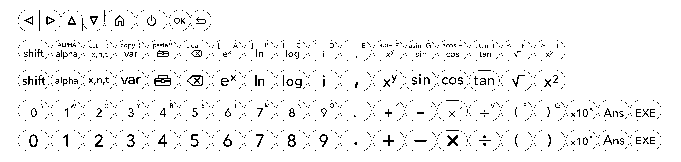
\includegraphics{calculatoritems-nwks-lua.pdf}
\end{DemoCode}

\pagebreak

\subsection{CASIO font, only with LUA/XE}

For \textsf{CASIO} models, there's \texttt{ttf} version of existing keys (\url{https://edu.casio.com/fr/forteachers/er/fontsets/}), and, with \ShowCode{[xelua]} loading option, it's possible to use \textit{directly} the font, defined with  \ShowCode{\\fontkeyCASIOcw} or \ShowCode{\\fontkeyCASIOfx} aliases, or with the macro for multiple keys.

\begin{DemoCode}{listing only}
%For CASIO classwiz, with availables symbols
{\fontkeyCASIOcw chars}
%For CASIO fx, with availables symbols
{\fontkeyCASIOfx chars}

%For CASIO classwiz, with availables aliases
\CalcKeyCasioCW{list of key, separated with +}
%For CASIO fx, with availables aliases
\CalcKeyCasioFX{list of key, separated with +}
\end{DemoCode}

\begin{DemoCode}{listing only}
\CalcKeyCasioCW{on+home+ok+up+down+left+right+pgup+pgdown+config+back}\\
\CalcKeyCasioCW{shift+var+fx+ctlg+tools+x+frac+sqrt+pow+sqr+exp+comma}\\
\CalcKeyCasioCW{sin+cos+tan+lp+rp+del+ac+times+div+plus+minus+sminus}\\
\CalcKeyCasioCW{1+2+3+4+5+6+7+8+9+0+dot+x10p+format+exe}\\
\CalcKeyCasioCW{semicol+ans}
\end{DemoCode}

\begin{DemoCode}{}
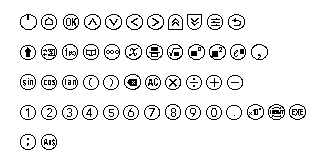
\includegraphics{calculatoritems-casiocw-lua.pdf}
\end{DemoCode}

\begin{DemoCode}{listing only}
\CalcKeyCasioFX{F1+F2+F3+F4+F5+F6+shift+optn+vars+menu}\\
\CalcKeyCasioFX{up+down+left+right+alpha+sqr+pow+exit}\\
\CalcKeyCasioFX{xtt+log+ln+sin+cos+tan+frac+sd+lp+rp+comma+sto}\\
\CalcKeyCasioFX{7+8+9+del+acon+4+5+6+times+div}\\
\CalcKeyCasioFX{1+2+3+plus+minus+0+dot+x10p+sminus+exe}
\end{DemoCode}

\begin{DemoCode}{}
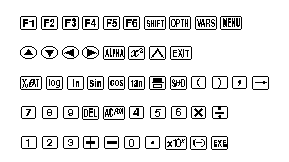
\includegraphics{calculatoritems-casiofx-lua.pdf}
\end{DemoCode}

\pagebreak

\subsection{Texas Instruments font, only with LUA/XE}

For \textsf{TI} models, there's \texttt{ttf} version of existing keys (\url{https://education.ti.com/en/software/search/key-fonts}), and, with \ShowCode{[xelua]} loading option, it's possible to use \textit{directly} the font, defined with \ShowCode{\\CalcKeyTI} or \ShowCode{\\CalcKeyTIfr} aliases, or with the macro for multiple keys.

\begin{DemoCode}{listing only}
%For TI84CE, with availables symbols
{\fontkeyTI chars}
%For TI83CE.fr, with availables symbols
{\fontkeyTIfr chars}

%For TI84CE, with availables aliases
\CalcKeyTI{list of key, separated with +}
%For TI83CE.fr, with availables aliases
\CalcKeyTIfr{list of key, separated with +}
\end{DemoCode}

\begin{DemoCode}{listing only}
\CalcKeyTI{y+window+zoom+trace+graph+2nd+mode+del+left+up+right+down}\\
\CalcKeyTI{alpha+xttn+stat+math+apps+prgm+vars+clear}\\
\CalcKeyTI{inv+sin+cos+tan+pow+sqr+comma+lp+rp+div}\\
\CalcKeyTI{log+7+8+9+times+ln+4+5+6+minus}\\
\CalcKeyTI{sto+1+2+3+plus+on+0+dot+sminus+enter}
\end{DemoCode}

\begin{DemoCode}{}
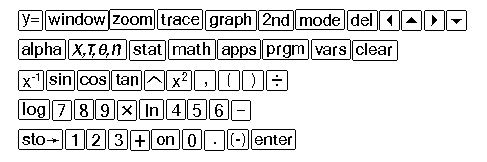
\includegraphics{calculatoritems-texas-lua.pdf}
\end{DemoCode}

\begin{DemoCode}{listing only}
\CalcKeyTIfr{fx+fenetre+zoom+trace+graphe+2nde+mode+supp+left+up+right+down}\\
\CalcKeyTIfr{alpha+xttn+stats+math+matrice+prgm+var+annul}\\
\CalcKeyTIfr{fmt+trig+resol+frac+pow+sqr+virg+lp+rp+div}\\
\CalcKeyTIfr{log+7+8+9+times+ln+4+5+6+minus}\\
\CalcKeyTIfr{sto+1+2+3+plus+on+0+dot+sminus+entrer}
\end{DemoCode}

\begin{DemoCode}{}
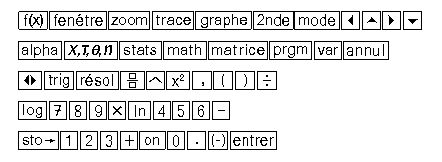
\includegraphics{calculatoritems-texasfr-lua.pdf}
\end{DemoCode}

\pagebreak

\subsection{Personal keys}

In order to use personal versions of keys (not included with the package, but available \href{https://packages.cpierquet.fr/packages/graphiques/calculatoritems/calculatoritems_keys.zip}{[here]}), you an use (internal) \ShowCode{\\inckeycalc} with \texttt{pdf/png/...} files named \texttt{calcitems\_<model>\_<key>.<ext>}.

\begin{DemoCode}{listing only}
%with personal keys, in an readable folder
\inckeycalc(*)[options]{model}{key}[extension]

%the starred version uses includegraphics, with optional arguments
%whereas the non starred uses inlinegraphics, with optional arguments (scale=... / strut=...)
\end{DemoCode}

\newcommand\insertcalckeys[2]{\Large\foreach \i in {#2}{\inckeycalc{#1}{\i}\relax}}

\begin{DemoCode}{listing only}
%loop for multiple keys
\newcommand\insertcalckeys[2]{%
	\foreach \i in {#2}{\Large\inckeycalc{#1}{\i}\relax}%
}
\end{DemoCode}

\begin{DemoCode}{}
%CASIO fx92 College CW (from svg)
\insertcalckeys{casio92cw}{on,home,config,back,ok}\\
\insertcalckeys{casio92cw}{left,up,right,down,pgud}\\
\insertcalckeys{casio92cw}{shift,var,fx,ctlg,tools}\\
\insertcalckeys{casio92cw}{x,frac,sqrt,pow,sqr,semicol}\\
\insertcalckeys{casio92cw}{rep,sin,cos,tan,lp,rp}\\
\insertcalckeys{casio92cw}{7,8,9,del,ac}\\
\insertcalckeys{casio92cw}{4,5,6,times,div}\\
\insertcalckeys{casio92cw}{1,2,3,plus,minus}\\
\insertcalckeys{casio92cw}{0,comma,x10p,fmt,exe}
\end{DemoCode}

\begin{DemoCode}{}
%CASIO graph light (from svg)
\insertcalckeys{casioglight}{on,home,config,back}\\
\insertcalckeys{casioglight}{left,up,right,down,pgud}\\
\insertcalckeys{casioglight}{shift,var,fx,ctlg,tools}\\
\insertcalckeys{casioglight}{x,frac,sqrt,pow,sqr,exp}\\
\insertcalckeys{casioglight}{comma,sin,cos,tan,lp,rp}\\
\insertcalckeys{casioglight}{7,8,9,del,ac}\\
\insertcalckeys{casioglight}{4,5,6,times,div}\\
\insertcalckeys{casioglight}{1,2,3,plus,minus}\\
\insertcalckeys{casioglight}{0,dot,x10p,fmt,exe}
\end{DemoCode}

\begin{DemoCode}{}
%CASIO graph math (from svg)
\insertcalckeys{casiogmath}{on,home,settings,back,next,prev}\\
\insertcalckeys{casiogmath}{left,up,right,down,pgud}\\
\insertcalckeys{casiogmath}{shift,alpha,var,ctlg,tools}\\
\insertcalckeys{casiogmath}{xtty,frac,sqrt,pow,sqr,exp}\\
\insertcalckeys{casiogmath}{comma,sin,cos,tan,lp,rp}\\
\insertcalckeys{casiogmath}{7,8,9,del,ac}\\
\insertcalckeys{casiogmath}{4,5,6,times,div}\\
\insertcalckeys{casiogmath}{1,2,3,plus,minus}\\
\insertcalckeys{casiogmath}{0,dot,x10p,fmt,exe}
\end{DemoCode}

\begin{DemoCode}{}
%CASIO graph35+e ii (from png)
\insertcalckeys{casio35p}{F1,F2,F3,F4,F5,F6}\\
\insertcalckeys{casio35p}{shift,optn,vars,menu}\\
\insertcalckeys{casio35p}{arrows}\\
\insertcalckeys{casio35p}{alpha,sqr,pow,exit}\\
\insertcalckeys{casio35p}{shift,optn,vars,menu}\\
\insertcalckeys{casio35p}{xtt,log,ln,sin,cos,tan}\\
\insertcalckeys{casio35p}{frac,sd,lp,rp,comma,sto}\\
\insertcalckeys{casio35p}{7,8,9,del,ac}\\
\insertcalckeys{casio35p}{4,5,6,times,div}\\
\insertcalckeys{casio35p}{1,2,3,plus,minus}\\
\insertcalckeys{casio35p}{0,dot,x10p,sminus,exe}
\end{DemoCode}

\begin{DemoCode}{}
%CASIO graph90 (from png)
\insertcalckeys{casio90p}{F1,F2,F3,F4,F5,F6}\\
\insertcalckeys{casio90p}{shift,optn,vars,menu}\\
\insertcalckeys{casio90p}{arrows}\\
\insertcalckeys{casio90p}{alpha,sqr,pow,exit}\\
\insertcalckeys{casio90p}{shift,optn,vars,menu}\\
\insertcalckeys{casio90p}{xtt,log,ln,sin,cos,tan}\\
\insertcalckeys{casio90p}{frac,sd,lp,rp,comma,sto}\\
\insertcalckeys{casio90p}{7,8,9,del,ac}\\
\insertcalckeys{casio90p}{4,5,6,times,div}\\
\insertcalckeys{casio90p}{1,2,3,plus,minus}\\
\insertcalckeys{casio90p}{0,dot,x10p,sminus,exe}
\end{DemoCode}

\begin{DemoCode}{}
%TI 83CEfr (from png)
\insertcalckeys{ti83ce}{fx,fenetre,zoom,trace,graphe}\\
\insertcalckeys{ti83ce}{arrows}\\
\insertcalckeys{ti83ce}{2nde,mode,suppr}\\
\insertcalckeys{ti83ce}{alpha,xttn,stats}\\
\insertcalckeys{ti83ce}{math,matrice,prgm,var,annul}\\
\insertcalckeys{ti83ce}{sd,trig,resol,frac,pow}\\
\insertcalckeys{ti83ce}{sqr,comma,lp,rp,div}\\
\insertcalckeys{ti83ce}{log,7,8,9,times}\\
\insertcalckeys{ti83ce}{ln,4,5,6,minus}\\
\insertcalckeys{ti83ce}{sto,1,2,3,plus}\\
\insertcalckeys{ti83ce}{on,0,dot,sminus,entrer}
\end{DemoCode}

\begin{DemoCode}{}
%TI 83CEfr full (from svg)
\insertcalckeys{ti83cefull}{fx,fenetre,zoom,trace,graphe}\\
\insertcalckeys{ti83cefull}{arrows}\\
\insertcalckeys{ti83cefull}{2nde,mode,suppr}\\
\insertcalckeys{ti83cefull}{alpha,xttn,stats}\\
\insertcalckeys{ti83cefull}{math,matrice,prgm,var,annul}\\
\insertcalckeys{ti83cefull}{sd,trig,resol,frac,pow}\\
\insertcalckeys{ti83cefull}{sqr,comma,lp,rp,div}\\
\insertcalckeys{ti83cefull}{log,7,8,9,times}\\
\insertcalckeys{ti83cefull}{ln,4,5,6,minus}\\
\insertcalckeys{ti83cefull}{sto,1,2,3,plus}\\
\insertcalckeys{ti83cefull}{on,0,dot,sminus,entrer}
\end{DemoCode}

\end{document}
